\documentclass[12pt, oneside]{article}
\usepackage{amssymb}
\usepackage{amsthm}	
\usepackage[centertags]{amsmath}
\usepackage{authblk}
\usepackage{booktabs}
\usepackage[labelfont=bf]{caption}
\usepackage{chngcntr}
\usepackage{color, soul}
\usepackage{float}
\usepackage[T1]{fontenc}
\usepackage[perpage]{footmisc}
\usepackage{fullpage}
\usepackage{fancybox}
\usepackage{geometry}                		
\usepackage{graphics}                		
\usepackage{graphicx}
\usepackage[utf8]{inputenc}
\usepackage{lineno}
\usepackage[]{microtype}
\usepackage[authoryear]{natbib}
\usepackage{placeins}
\usepackage{setspace}
\usepackage{textcomp}
\usepackage{textgreek}
\usepackage{threeparttable}
\usepackage[hyphens,spaces,obeyspaces]{url}
\usepackage{wrapfig}

%% Bibliography

\bibpunct{(}{)}{,}{a}{}{;} 
\renewcommand\refname{\textsc{References}} %renames Bibliography as References

\DeclareRobustCommand{\firstsecond}[2]{#1}

\newcommand{\mb}{\mathbf}
\newcommand{\bs}{\boldsymbol}
\newcommand{\wt}{\widetilde}
\newcommand{\s}{^{(\bss)}}
\newcommand{\bss}{\boldsymbol{s}}

% For Icelandic ð symbol:
\DeclareTextSymbolDefault{\dh}{T1}

\title{Estimating primary production in lakes: Comparison of \textsuperscript{14}C incubation and free-water O\textsubscript{2} approaches}

\author[1]{Noah R. Lottig\footnote{Corresponding author: nrlottig@wisc.edu}}
\author[2]{Joseph Phillips}
\author[3]{Ryan D. Batt}
\author[4]{Facundo Scordo}
\author[5]{Tanner J. Williamson}
\author[6]{Stephen R. Carpenter}
\author[4] {Sudeep Chandra}
\author[6]{Paul C. Hanson}
\author[7]{Chistopher T. Solomon}
\author[5] {Michael J. Vanni}
\author[8]{Jacob Zwart}


\affil[1]{University of Madison Center for Limnology, Boulder Junction, Wisconsin 54512 USA}
\affil[2]{Department of Aquaculture and Fish Biology, H\'{o}lar University, Skagafj\"{o}r{\dh}ur 551 Iceland}
\affil[3]{Rutgers University, New Brunswick, New Jersey}
\affil[4]{University of Nevada, Reno, Reno Nevada}
\affil[5]{Department of Biology, Miami University, Oxford, Ohio }
\affil[6]{University of Madison Center for Limnology, Madison, Wisconsin 53706 USA}
\affil[7]{Cary Institute of Ecosystem Studies, Millbrook, New York}
\affil[8]{Integrated Information Dissemination Division, U.S. Geological Survey, South Bend, Indiana 46617 USA}

\geometry{letterpaper,total={6.5in,9in},}   
\begin{document}
\maketitle

\noindent {\bf Data availability statement}: All data and code available for peer review at: location. Data will be made public with associated DOI if/when the manuscript is accepted and finalized.
\vspace{\baselineskip}

{\bf \noindent Keywords}: lake, production, metabolism, gross primary production, \textsuperscript{14}C incubations, dissolved oxygen, GPP
\vspace{5mm}

{\bf \noindent Running Header}: Comparing \textsuperscript{14}C and in situ O\textsubscript{2} primary production estimates
\vspace{5mm}

\textit{This draft manuscript is distributed solely for the purposes of scientific peer review. Its content is deliberative and predecisional, so it must not be disclosed or released by reviewers. Because the manuscript has not yet been approved for publication by the U.S. Geological Survey (USGS), it does not represent any official USGS finding or policy.}


\newpage
\doublespacing
\linenumbers

%----------------------------------------ABSTRACT-----------------------------------------%
\section*{Abstract}
Historically, estimates of pelagic primary production in aquatic ecosystems were made by measuring the uptake of \textsuperscript{14}C labeled inorganic carbon in samples incubated under laboratory or in situ conditions.  More recently, incubation approaches have been increasingly replaced by methods that leverage diel changes in high-frequency in situ data such as free-water dissolved oxygen (O\textsubscript{2}). While there is a rich history of comparing different approaches for estimating primary production using incubations (e.g., \textsuperscript{14}C and O\textsubscript{2} bottle experiments) or more recently high-frequency data (e.g., diel O\textsubscript{2} and CO\textsubscript{2} metabolism models), direct comparisons of \textsuperscript{14}C incubations and free-water O\textsubscript{2} approaches for estimating primary production are limited. We leveraged 20 lake-years of concurrent measurements of primary production quantified from high frequency free-water O\textsubscript{2} data and \textsuperscript{14}C incubations in four different lakes (4 - 7 years per lake) to compare these different approaches for estimating pelagic lake primary production. Across all lakes, 61\% of the \textsuperscript{14}C production estimates were contained within the 95\% credible intervals of the free-water O\textsubscript{2} production estimates. Error-in-variable regressions suggest that the data are consistent with the well-accepted assumption that \textsuperscript{14}C methods estimate a production value between gross primary production and net primary production, but the bottle effect is constant across the entire range of production values considered here. Overall, results of these analyses provide little evidence that pelagic, epilimnetic estimates of daily lake primary production differ substantially based on the selection of free-water O\textsubscript{2} or \textsuperscript{14}C approaches and that these two approaches are largely interchangeable across the ranges of productivity considered here. 

\vspace{\baselineskip}
\newpage

%------------------------------------INTRODUCTION-----------------------------------------%
\section*{Introduction}
\label{S:1}
Primary production, the production of organic matter by autotrophs, is a fundamental process that in most ecosystems determines the amount of energy available to higher trophic levels.  In the pelagic regions of lakes and reservoirs, oxygenic primary production is typically determined using variants of two basic techniques:  measuring the uptake of dissolved inorganic carbon or the production of dissolved oxygen (\citealt{hall_measuring_2007}, but see \citealt{peeters_lake_2016,peeters_calculation_2019} as examples of other approaches). These techniques can be applied either in situ or in laboratory incubations and can include measurements in bottles or open water.

Primary production measurements using uptake of inorganic carbon usually involve spiking a sample of lake water with a known amount of inorganic \textsuperscript{14}C, incubating the spiked sample under known temperature and light conditions (either in the lake or in the laboratory), and measuring the amount of labeled carbon that is fixed into organic forms by algae via photosynthesis during the incubation \citep{Fee_1973,peterson_aquatic_1980}.  This technique has multiple advantages.  The \textsuperscript{14}C technique can be used in low production systems because the abundance of \textsuperscript{14}C can be measured precisely \citep{hall_measuring_2007}.  Samples can be incubated at multiple light levels allowing calculation of production versus light relationships that can be used to estimate pelagic primary production at multiple depths in the lake.  Repeated measurements within a year allow for the estimation of annual primary production and similarly long-term trends in primary production.  For these reasons many research programs have compiled long time series of production measurements based on this technique.

The \textsuperscript{14}C approach poses some challenges. First, this approach estimates production only of the water placed in the bottle under the environmental conditions in which it is incubated. Consequently, extrapolating production to a region of the lake or the whole ecosystem entails assumptions about the representativeness of those incubations for the region to which they are being extrapolated. Further, because some carbon fixed during the incubation can be respired \citep{Vollenweider_Talling_Westlake_1974, peterson_aquatic_1980}, the technique is commonly presumed to underestimate gross primary production (GPP) and may be closer to Net Primary Production (NPP). The magnitude of the underestimation is dependent on incubation time and algal turnover rates \citep{hall_measuring_2007}, although there are approaches to account for this underestimation \citep{Legendre_Demers_Yentsch_Yentsch_1983}. Additionally, due to costs, time-consuming nature of the incubations, and the  fact that approach generates radioactive waste, research projects are often limited in the frequency at which production estimates can be made. Nonetheless, this technique has been the standard by which all other approaches have been compared \citep{peterson_aquatic_1980}.

More recently, free-water (e.g., \citealt{Vachon_Sadro_2020}) dissolved oxygen (O\textsubscript{2}) techniques have emerged as a common approach to estimate production of aquatic ecosystems  because the data can be readily obtained at high frequencies using in situ sensors in contrast to the \textsuperscript{14}C approach . While O\textsubscript{2} techniques have long been used to estimate production in aquatic systems \citep{Sargent_Austin_1949, Odum_1956,staehr_lake_2010}, the advent of automated sensors capable of making in situ, high frequency measurements of O\textsubscript{2} greatly reduced the labor associated with this technique along with providing opportunities to gather the data during hard to sample time points such as storm events or ice breakup as examples. Several models can be used to estimate metabolism from sensor data
\citep{Cole_Pace_Carpenter_Kitchell_2000, Hanson_Carpenter_Kimura_Wu_Cornelius_Kratz_2008, Holtgrieve_Arias_Irvine_Lamberts_Ward_Kummu_Koponen_Sarkkula_Richey_2013, Batt_Carpenter_2012, solomon_ecosystem_2013, phillips_timevarying_2020}. These approaches all assume that biological production and atmospheric exchange drive changes in oxygen \citep{Odum_1956}. A major advantage of the free-water O\textsubscript{2} approach is that it allows multiple components of metabolism (GPP, ecosystem respiration [R], and net ecosystem production [NEP]) to be estimated simultaneously. Additionally, free-water O\textsubscript{2} metabolism estimates can integrate across habitats (e.g., benthic and pelagic production) when the sensor is located in a well-mixed parcel of water that is in contact with these habitats \citep{VandeBogert_Carpenter_Cole_Pace_2007}.  Because of the relative ease of measurement using this technique, many research groups, such as those in the Global Lake Ecological Observatory Network (GLEON; \citealt{Weathers_Hanson_2013}) have adopted this technique \citep{solomon_ecosystem_2013}. On the other hand, estimates based on the free-water O\textsubscript{2} approach can be difficult to interpret because metabolic rates exhibit substantial vertical \citep{Staehr_Christensen_Batt_Read_2012} and horizontal \citep{VandeBogert_Bade_Carpenter_Cole_Pace_Hanson_Langman_2012} heterogeneity within a lake, and movement of water parcels past the sensor can cause oxygen levels recorded by the sensor to change even in the absence of biological processes. Furthermore, how models account for physical gas exchange (e.g., \citealt{dugan_consequences_2016}) along with the spatial differences in processes can lead to noisy high-frequency observations \citep{Batt_Carpenter_2012} or to large and significant changes in estimated metabolism rates between days \citep{solomon_ecosystem_2013}. Therefore, heterogeneity complicates the interpretation of the results and potentially compromises their accuracy at short temporal time scales.

As the free-water O\textsubscript{2} and other approaches that leverage high-frequency in situ data continue to gain popularity, much is yet to be learned about how these estimates compare to those from \textsuperscript{14}C incubations. There is a long history of comparing \textsuperscript{14}C incubations to O\textsubscript{2} production from light/dark bottle incubations to determine production levels in marine and aquatic environments \citep{Williams_Heinemann_Marra_Purdie_1983, Bender_Grande_1987, Gazeau_Middelburg_Loijens_Vanderborght_Pizay_Gattuso_2007}. Similarly, studies in marine systems have compared \textsuperscript{14}C incubations to steady-state, sample-based oxygen methods like \textsuperscript{18}O labeling, triple-isotope, \textsuperscript{17}$\Delta$, O\textsubscript{2}/Ar, and others, and have generally found that the \textsuperscript{14}C methods produce lower estimates \citep{juranek_vitro_2005, quayetal2010, Hamme_Cassar_2012,Regaudie_2014}. To our knowledge, no direct comparison of the free-water O\textsubscript{2} and bottle \textsuperscript{14}C methods across multiple lakes and years have been made (but see \citealt{lauster_gross_2006} for free-water and O\textsubscript{2} bottle comparisons). Here we use 20 lake-years of data from four lakes of varying trophic status to assess how similar in situ free-water O\textsubscript{2} pelagic epilimnetic production estimates are to concurrent pelagic epilimnetic estimates made using \textsuperscript{14}C incubations. 

%---------------------------------------METHODS-------------------------------------------%
\section*{Materials and Procedures}
\subsection*{Study Lakes} %---------------------------Study Lakes-------------------------%

Daily lake \textsuperscript{14}C pelagic production, high-frequency dissolved oxygen (O\textsubscript{2}), water temperature, and meteorological data were collected as part of an ongoing long-term research projects in northern Wisconsin (North Temperate Lakes [NTL] Long-Term Ecological Research Program\footnote{lter.limnology.wisc.edu}; Trout and Sparkling Lakes), California (Castle Lake Environmental Research and Education Program\footnote{aquaticecosystemslab.org/projects/castlelake}; Castle Lake), and Ohio (Center for Aquatic \& Watershed Sciences\footnote{miamioh.edu/cas/academics/centers/caws}; Acton Lake). Sparkling and Trout lakes are embedded in a landscape that is predominantly a mix of deciduous and coniferous forest (54\%), lakes (13\%), and wetlands (28\%) \cite{magnuson_long-term_2006}. Both study lakes are oligotrophic/mesotrophic with relatively low nutrient and chlorophyll concentrations (Table \ref{tab:table1}). Castle Lake is a meso-oligotrophic, subalpine (1646 m. a.s.l.) lake \citep{VanderZanden_Chandra_Park_Vadeboncoeur_Goldman_2006} located in northern California with similar nutrient and chlorophyll concentrations as Trout and Sparkling lakes (Table \ref{tab:table1}). Acton Lake is a hypereutrophic reservoir (Table \ref{tab:table1}) that was created in 1957 by damming a creek for recreational use. Watershed landuse is primarily row crop agriculture ($>$80\%, \citealt{vanni_dissolved_2001}).

\subsection*{\textsuperscript{14}C Production Methods} %---------C14 methods--------------%

The approaches for estimating primary production in the study lakes using \textsuperscript{14}C incubations differed slightly between the three research programs, but all resulted in a similar estimate of daily epilimnetic pelagic production (mmol C m\textsuperscript{-3} d\textsuperscript{-1}). In NTL lakes, vertical cores (i.e., integrated samples) of water from the surface of the lake to the bottom of the epilimnion were collected between 2007 and 2013 using a 1.5 inch PVC tube approximately every two weeks during the open water season (first described in these lakes by \citealt{adams_primary_1993}). Samples were labeled with inorganic \textsuperscript{14}C in the form of NaHCO\textsubscript{3} and then incubated in the lab for 3-hr across a range of light intensities with additional dark bottles to correct for non-uptake sorption of \textsuperscript{14}C at ambient epilimnetic water temperature. The resultant photosynthesis-irradiance (P-I) data was used to derive P-I curves by fitting a 3-parameter photosynthesis light-inhibition model \citep{Platt_Gallegos_Harrison_1980} to these data. The P-I curves were coupled with concurrent, high-frequency photosynthetically active radiation ($\mu$mol m\textsuperscript{-2} s\textsuperscript{-1}; PAR) measurements and water column light extinction data (m\textsuperscript{-1}) to estimate daily primary production (mmol C m\textsuperscript{-3} d\textsuperscript{-1}) in both Sparkling and Trout Lake. Over this time period, the availability of data for \textsuperscript{14}C production varied due to sporadic sample contamination and equipment failures.

At Castle Lake, vertical water collections were made from 13 depths between the surface and 30 m; duplicate light and 1 dark bottle samples from each each depth were labeled with inorganic \textsuperscript{14}C in the form of NaHCO\textsubscript{3} and then incubated in situ at the depth of collection for 4 hours. Detailed methods are described elsewhere \citep{Goldman_Mason_Wood_1963, Goldman_1968}. Total daily incident solar radiation was measured throughout the summer with a LI-COR Li-200 pyrheliometer. Light profiles at the height of the solar day are measured using a Biospherical Instruments 2104P radiometer. Daily phytoplankton productivity rates were calculated by dividing productivity measured during the incubation period by the fraction of the total daily PAR received during the incubation.

Methods for \textsuperscript{14}C incubations in Acton Lake were similar to those in NTL lakes. Integrated samples were collected from the euphotic zone (usually equal to the epilimnion) and incubated in the lab for 1-2 hr with NaHCO\textsubscript{3} at a range of light intensities (including dark bottles; \citealt{fee1990computer}). Incubations were usually done every two weeks (23 of 55 experiments over the four years) or more frequently (24 experiments); only 8 experiments were done at intervals >2 weeks. As in NTL lakes, P-I curves were coupled with high-frequency PAR  measurements, and water column light extinction data collected at weekly intervals. Detailed methods \textsuperscript{14}C are described in \citet{Knoll_Vanni_Renwick_2003}.  

%------------------------------------O2 Metabolism---------------------------------------%
\subsection*{Free-water O\textsubscript{2} Metabolism Methods}

The same approach was used to estimate pelagic primary production (mmol C m\textsuperscript{-3} d\textsuperscript{-1}; GPP) in all lakes using in situ time series of dissolved oxygen data (O\textsubscript{2}). Free-water O\textsubscript{2} production estimates were based on high frequency measurements of dissolved oxygen (mg L\textsuperscript{-1}), water temperature (\textcelsius{}), PAR ($\mu$mol m\textsuperscript{-2} s\textsuperscript{-1}), wind speed (m s\textsuperscript{-1}), and barometric pressure (mbar). Data frequencies varied from 1 to 15 minutes based on the research program and the year data was collected. The raw, high-frequency time series of dissolved oxygen and water temperature were filtered to remove outliers by excluding values that were greater than 3 and 5 standard deviations respectively from a 7-day running average (Appendix \ref{Appendix:appendix_trimmed}A,B; \emph{sensu} \citealt{phillips_timevarying_2020}). The choice of sampling frequencies has implications for the processes influencing dissolved oxygen patterns and the amount of data needed to characterize those processes \citep{staehr_lake_2010}. In general, frequencies between 30 minutes and 3 hours are optimal for capturing changes driven by biological processes \citep{staehr_lake_2010}. Thus, we extracted hourly time series for all high frequency data by averaging observations (mean value) on the hour of observation (n = 4-60 depending on frequency of raw data) centered on the hour \citep{phillips_timevarying_2020} for use in metabolism models.

Epilimnetic depth (m) was quantified from either high-frequency thermistor string data (Trout, Sparkling, and Acton Lakes) or discrete temperature profiles (Castle Lake). The high frequency data was filtered for outliers as outlined above and epilimnetic depth determined using the rLakeAnalyzer package \citep{read_derivation_2011, winslow_rlakeanalyzer_2019} at the temporal frequency of the raw data. Hourly aggregate data was then extracted based on a 1-day running average to reduce the significant amount of noise that existed in these estimates (Appendix \ref{Appendix:appendix_trimmed}C). rLakeAnalyzer was also used to quantify epilimnetic depth from bi-monthly water temperature profile data in Castle Lake and linearly interpolated at hourly time steps between observations.

Exchange of dissolved gas with the atmosphere is a critical component of metabolism models, and, while there are a number of different models for estimating piston velocities in lentic ecosystems \citep{dugan_consequences_2016}, the model proposed by \citealt{vachon_ecosystem_2013} is robust across multiple different types of lakes \citep{dugan_consequences_2016} and the metabolism model leveraged in this study (see below) is quite robust to choice in parameterization of piston velocities \citep{phillips_timevarying_2020}. Piston velocities (m hr\textsuperscript{-1}) were calculated using the LakeMetabolizer R package \citep{winslow_lakemetabolizer_2016} and the parameterization proposed by \citealt{vachon_ecosystem_2013}. Light extinction coefficients (m\textsuperscript{-1}), which were typically quantified bimonthly in all lakes, were linearly interpolated at hourly time steps between observations, combined with epilimnetic depth, and PAR to estimate the average light levels within the epilimnion of each lake \citep{staehr_lake_2012,phillips_timevarying_2020}

The data described above were used to generate daily estimates (mmol O\textsubscript{2} m\textsuperscript{-3} d\textsuperscript{-1}) of gross primary production (GPP), respiration (R), and net ecosystem production (NEP) using a time-varying ecosystem metabolism model \citep{phillips_timevarying_2020}. This model differs from many of the more commonly used metabolism models (e.g., \citealt{winslow_lakemetabolizer_2016}) in that the model is not fit iteratively over a daily time scale, but rather characterizes changes across all time periods (hourly measurements across 4-7 years of data) for a given lake in a single model fit, as well as constraining GPP and respiration to positive and negative values respectively (i.e., ecologically feasible ranges; \citealt{phillips_timevarying_2020}). This takes advantage of the fact that the physical and biological processes governing ecosystem metabolism and other aspects of DO dynamics are autocorrelated through time, which means that this shared information can be used to inform the parameter estimates across all time points. Furthermore, this method is statistically unified because it uses all data to fit a single model, which facilitates characterizing the uncertainty in the ecosystem metabolism estimates \citep{phillips_timevarying_2020}. 


The model used here differs slightly from that presented in \citealt{phillips_timevarying_2020} in that we used a photoinhibition P-I curve \citep{steele_environmental_1962} to describe GPP (\emph{sensu} \citealt{staehr_global_2016}) instead of a light saturating curve: 
\[
P_I = P_{max} \frac{I}{I_{opt}} \exp\left(1-\frac{I}{I_{opt}} \right)
\]
where \(P_I\) is the production rate at light intensity \emph{I}, \(P_{max}\) is the maximum production rate, and \(I_{opt}\) is the optimal light intensity. This photoinhibition model was chosen because recent work by \citet{staehr_global_2016} found that photoinhibition in lakes was common, the \citet{steele_environmental_1962} is one of the simplest photoinhibition models (two-parameter), and, regardless of the P-I curve formulation chosen, it is often difficult to distinguish significant differences in model fits between different models \citep{Aalderink_Jovin_1997}. Both \(P_{max}\) and \(I_{opt}\) were allowed to vary through time at a daily time scale.

Observed dissolved oxygen time series were fit to all years (Trout: 2007-2010, 2012; Sparkling: 2007-2013; Castle: 2014-2017; Acton: 2010-2012, 2014) simultaneously for each lake individually (i.e., lake specific metabolism model fitting). The presence of missing values in the model input data time series meant that some days had less than 24 observations. Although the metabolism model can deal with missing data because it fits the entire time series simultaneously instead of in discrete daily time steps, we did not estimate metabolism parameters for a individual day if more than two hours of data was missing for that day \citep{phillips_timevarying_2020}. The model was fit via Stan (GET VERSION) run in R (GET VERSION) using the rstan package (STAN Citation) as described in \citep{phillips_timevarying_2020}. Posterior median values were used for daily production values along with the 0.025 and 0.975 quantiles of the posterior values to characterize the 95\% credible intervals. Model fits were validated by checking effective sample size, $\hat{R}$, tree depth, energy Bayesian Fraction of Missing Information, and divergence (see \citealt{betancourt_robust_2007}). Estimates of any metabolism parameters were not made when the epilimnetic depth was shallower than the dissolved oxygen sensor ($<$0.5m in Trout, Sparkling, Acton; $<$3m Castle; 4\% of all observations). Gross primary production values (mmol O\textsubscript{2} m\textsuperscript{-3} d\textsuperscript{-1}) were converted to units of carbon (mmol C m\textsuperscript{-3} d\textsuperscript{-1}) assuming a photosynthetic quotient (O\textsubscript{2}:CO\textsubscript{2}) of 1.25 \citep{bott_primary_1996,hanson_lake_2003,wielgat-rychert_calculation_2017}. 

Data and code associated with the analyses included in this manuscript (Lottig et al. reference updated upon acceptance)

%--------------------------------------------------Results--------------------------------------------------------%
\section*{Assessment}

The goal of the analyses presented here is to compare \textsuperscript{14}C and in situ free-water O\textsubscript{2} daily primary production estimates to determine how interchangeable these two approaches are. We specifically tailor our analyses to identify two potential biases. First, given the commonly presumed  bias of \textsuperscript{14}C to slightly lower than GPP \citep{peterson_aquatic_1980,hall_measuring_2007}, we wanted to know if there are constant differences in the magnitude of daily production values between the two approaches (i.e., we expected free-water O\textsubscript{2} approach to yield higher estimates than the \textsuperscript{14}C approach). Second, we wanted to know if there were any fixed biases (i.e., intercept of linear regression different from zero) and/or proportional biases between the two methods (i.e., slope of linear regression different from 1). A priori, we assumed that free-water O\textsubscript{2} estimates of GPP should be slightly higher than \textsuperscript{14}C (i.e., fixed bias) but the two methods should yield proportionally similar results. If there were no significant fixed or proportional biases, we interpret the results to mean that the methods are interchangeable for the lakes considered in this study.

Across the four lakes included in this study, we had 20 lake-years of concurrent \textsuperscript{14}C and free-water O\textsubscript{2} pelagic, epilimnetic primary production estimates (Acton Lake: 4 yrs, Castle Lake: 4 yrs, Sparkling Lake: 7 yrs, Trout Lake: 5 yrs, Fig. \ref{fig:timeseries}) where direct comparisons between production estimates were available on 101 discrete days. In most cases (61\%; 75\% excludint Castle Lake) , \textsuperscript{14}C estimates of production were contained within the 95\% credible intervals of the free-water O\textsubscript{2} estimates and the seasonal patterns were similar between the two approaches (Fig. \ref{fig:timeseries}, but see Castle Lake). 

To assess potential biases between free-water O\textsubscript{2} and \textsuperscript{14}C daily production estimates, epilimnetic production was compared by regressing \textsuperscript{14}C daily production values against free-water O\textsubscript{2} daily production values. We assume that a slope of one and intercept of zero indicates that no significant difference exists between the two approaches (i.e., the methods are interchangeable). Intercept values significantly different from zero would indicate potential fixed biases, and slope values significantly different than one would indicate a proportional bias. Because both \textsuperscript{14}C and O\textsubscript{2} estimates contain measurement errors \citep{macedo_annual_2001,pemberton_quantifying_2006,solomon_ecosystem_2013}, we used robust principal components error-in-variables regression \citep{passing_new_1983} implemented in the 'mcr' r package \citep{manuilova_mcr_2014}. While the data were log-transformed in some cases prior to analysis to increase the normality of the observations, we also include results from regressions on non-log-transformed data. 

A strong linear relationship was observed between the two approaches for estimating in-lake production across the approximate 200 mmol C m\textsuperscript{-3} d\textsuperscript{-1} pelagic epilimnetic production gradient observed in this study (Fig. \ref{fig:pointestimates}). Error in variable regression using all discrete observations (n=101) included the line of equality suggesting across large gradients of pelagic epilimnetic production, there was no proportional difference between the two approaches for measuring production in the lakes examined here (Table \ref{tab:table2}). The slight rightward shift in the distribution of free-water O\textsubscript{2} as well as an intercept significantly greater than 0 in the error-in-variables (log transformed) regression is consistent with the general assumption that \textsuperscript{14}C production methods typically quantify a value slightly lower than GPP \citep{peterson_aquatic_1980,hall_measuring_2007}. The linear relationships between the two approaches were consistent regardless if the data were log-transformed or not (Table \ref{tab:table2}). The increase in slope coefficient values in the non-logged analyses for all lakes is largely due to the low productivity systems serving as a leverage point in the regression. Confidence intervals of  non-transformed error in variable regression for Acton Lake (high productivity) and low productivity lakes included the line of equality (Table \ref{tab:table2}).

At a lake-specific level, the linear 1:1 patterns are not as strong in each lake as those observed both across lakes and across wide gradients in pelagic epilimnetic production (Fig. \ref{fig:lakevalues}, Table \ref{tab:table3}). For example, in Trout Lake there is actually a significant negative relationship (Table \ref{tab:table3}. However, the lack of a strong 1:1 linear relationship is likely driven in large part by the limited range of observed production values within a given lake combined with the uncertainty of both \textsuperscript{14}C (unknown) and free-water O\textsubscript{2} production estimates (quantified). Despite the narrow range of \textsuperscript{14}C production observed in the different lakes, most of the points cluster around the 1:1 line and a majority (61\%; 75\% excluding Castle Lake) of the 95\% credible intervals of the free-water O\textsubscript{2} estimates intersect the 1:1 line. Finally, Castle Lake is unique relative to the other three lakes considered in this study in that the data suggests a consistent lower production (1.7 mmol C m\textsuperscript{-3} d\textsuperscript{-1}) value estimated with the \textsuperscript{14}C approach relative to the free-water O\textsubscript{2} approach (Table \ref{tab:table3}).

Free-water O\textsubscript{2} metabolism estimates can vary substantially from day to day \citep{Staehr_Sand-Jensen_2007, staehr_lake_2010, Coloso_Cole_Pace_2011, VandeBogert_Bade_Carpenter_Cole_Pace_Hanson_Langman_2012, solomon_ecosystem_2013}. As with many other studies, the daily time series of O\textsubscript{2} daily production in this study exhibited high day-to-day variation, especially in the hypereutrophic system (Acton Lake; \ref{fig:timeseries}). Because both spatial and temporal averaging can reduce variability in metabolism estimates \citep{staehr_lake_2010, VandeBogert_Bade_Carpenter_Cole_Pace_Hanson_Langman_2012, Richardson_Carey_Bruesewitz_Weathers_2017, Zwart_Sebestyen_Solomon_Jones_2017}, we explored whether averaging (median value) free-water daily production estimates over 7 days (weekly) centered on the day of \textsuperscript{14}C incubations strengthened the relationship between O\textsubscript{2} daily production and \textsuperscript{14}C daily production. Overall, comparing \textsuperscript{14}C estimates to the median value of O\textsubscript{2} production did not alter the conclusions drawn from comparing measurements made on the same day, but the results suggest that comparing the weekly median value reduced any proportional bias in the data and increased the likelihood of a magnitude bias in the data as we and others hypothesized might exist (Table \ref{tab:table3}, Fig. \ref{fig:medianvalues}).

%--------------------------------------------------Discussion--------------------------------------------------------%
\section*{Discussion}

Overall, the results from this study suggest that the pelagic, epilimnetic \textsuperscript{14}C and free-water O\textsubscript{2} production approaches examined here can be interpreted similarly for the lakes considered in this study. Across gradients in production from oligotrophic to hypereutrophric systems, both of these approaches provide production estimates that are very similar in magnitude. Comparison of results between both methods indicated no statistically significant deviation from the 1:1 relationship, although there is evidence that, as expected, \textsuperscript{14}C estimates may be slightly lower than free-water O\textsubscript{2} estimates of pelagic epilimnetic production. Unlike other studies (e.g., \citealt{staehr_lake_2010}), temporal aggregation of free-water O\textsubscript{2} estimates did not have a major impact on the relationships observed in this study, likely because the metabolism model smooths parameters estimates through time \citep{phillips_timevarying_2020}.

A priori, we anticipated that proportionally, free-water O\textsubscript{2} estimates would be similar to \textsuperscript{14}C estimates, but that \textsuperscript{14}C estimates would be, on average, slightly lower than free-water O\textsubscript{2} because \textsuperscript{14}C estimates tend to lie between GPP and net primary production (NPP; \citealt{peterson_aquatic_1980}). In general, the results of these analyses confirm our a priori expectations. The lack of strong statistical evidence across all lakes of lower \textsuperscript{14}C relative to O\textsubscript{2} estimates in our study may reflect the fact that there is considerable uncertainty in both estimates, which we explicitly incorporated in our analysis via the error-in-variables approach. Additionally, the research programs responsible for generating the \textsuperscript{14}C production estimates specifically targeted short incubation periods to generate estimates that closely approximated GPP \citep{hall_measuring_2007}. Thus, even though we observed slight lower \textsuperscript{14}C production estimates relative to the free-water O\textsubscript{2} estimates, the lack of strong statistical significance across all analyses is not necessarily surprising given approaches employed by the research programs collecting the \textsuperscript{14}C production data.

On an individual lake basis, Castle Lake is the exemption to the general conclusions drawn above when considering the relationships between the two approaches in all lakes simultaneously. There is strong evidence that, although the two approaches are proportionally similar, \textsuperscript{14}C estimates are significantly lower than free-water O\textsubscript{2} estimates for this lake alone. We believe there are two potential reasons for pattern in Castle Lake, one consistent with hypotheses presented here and one methodological. First, the degree to which \textsuperscript{14}C production estimates approximate GPP relative to NPP is influenced in part by the length (time) of incubations \citep{hall_measuring_2007} whereby shorter incubations tend to estimate a value closer to GPP or in the case of this study, free-water O\textsubscript{2} estimate. Castle Lakes incubations were the longest ($\sim$4 hours) of any of the three programs that collected \textsuperscript{14}C data and thus it might be expected that the relative differences between the approaches was greatest for this program relative to the other two programs that collect \textsuperscript{14}C data. The other potential issue relates to how the \textsuperscript{14}C data from Castle Lake were generated (see above). Briefly- samples were incubated in situ for 4 hours from 10:00 - 14:00 hours (time period of maximum solar insolation) and the relationship (i.e., P-I curve) between production and solar insolation was assumed to be linear when in reality the pattern is likely either light saturating or photoinhibiting. Because the the incubations were conducted when solar insolation was near maximal, this approach has the potential to significantly underestimate production rates at lower light levels regardless of the shape of the true P-I curve. The lowest \textsuperscript{14}C epilimnetic production estimates in Castle Lake were almost universally observed in samples that were incubated directly at the surface of the lake which receives that greatest amount of solar insolation relative to samples incubated at deeper depths and would be consistent with P-I curves characterized by strong photoinhibition. Thus, while not influencing the overall patterns across all lakes, Castle Lake serves as a strong reminder that it will be important to account for potential differences in how both \textsuperscript{14}C and free-water O\textsubscript{2} production data are generated.

While we suggest that free-water O\textsubscript{2} and \textsuperscript{14}C epilimnetic daily pelagic production approaches are largely interchangeable, it is important to emphasize that there is still substantial variability between the methods. The variability between approaches is partly explainable because it can be challenging to pull out a biological signal from small fluctuations in diel oxygen concentrations with the free-water method, since physical processes influencing O\textsubscript{2} dominate and/or errors in accounting for physical processes influencing O\textsubscript{2} make it difficult to fit metabolism models. Physical processes are less of a concern for incubations, although there are a whole suite of concerns with respect to bottle incubations \citep{hall_measuring_2007}. At the hypereutrophic end of the spectrum, high variability in daily free-water O\textsubscript{2} estimates are not unexpected \citep{Williamson_Vanni_Renwick_2020}, and bottle incubations for \textsuperscript{14}C production may miss important temporal and/or spatial variability that is captured by the free-water O\textsubscript{2} approach. Although averaging free-water production estimates did not alter the relationships observed between \textsuperscript{14}C and free-water O\textsubscript{2} production in the systems considered here, averaging free-water did reduce the variability around the line of equality (see Fig. \ref{fig:medianvalues}). Thus, averaging free-water O\textsubscript{2} production estimates over several days may increase the precision of these estimates relative to the \textsuperscript{14}C approach, especially in more productive systems.

Estimating metabolism parameters, including primary production from free-water O\textsubscript{2} data can be challenging in low productivity systems (e.g., \citealt{Richardson_Carey_Bruesewitz_Weathers_2017, McNair_Sesselmann_Kendall_Gereaux_Weinke_Biddanda_2015, Honti_Istvanovics_2019}) where \textsuperscript{14}C is generally considered optimal \citep{hall_measuring_2007}. Given that a majority of the lakes in this study are characterized by low productivity, it is likely that the ability of the \citep{phillips_timevarying_2020} model to leverage all possible data across multiple years to fit the models contributed to our ability generate production estimates in these systems that were consistent with \textsuperscript{14}C estimates. While not the focus of this study, there are opportunities with data such as these to explore how different free-water O\textsubscript{2} models perform and gain a better understanding of when and where different model formulations should be leveraged (e.g., \citealt{Honti_Istvanovics_Staehr_Brighenti_Zhu_Zhu_2016,staehr_global_2016, McNair_Sesselmann_Kendall_Gereaux_Weinke_Biddanda_2015}).

Analyses such as this are critical for gaining a better understanding of lake daily production measurements generated by these two widely used methods. Each method has unique advantages and disadvantages that may influence the choice of methods for particular research applications. For example, we would expect large differences between free-water and bottle estimates in freshwaters where littoral and benthic production contribute substantially to total metabolism \citep{lauster_gross_2006, VandeBogert_Carpenter_Cole_Pace_2007}. Thus, it is likely that both methods will continue to be used and there will be an ongoing need to compare results across methods. Analyses conducted here provide little evidence of systematic differences in estimates of epilimnetic lake daily production based on free-water O\textsubscript{2} or \textsuperscript{14}C methods across a wide gradient in lake trophic status.



%--------------------------------------------------Bibliography--------------------------------------------------------%
\newpage
\bibliographystyle{aslo.bst}
\bibliography{references.bib}

\clearpage
\section*{Acknowledgements}
Data collection and analysis was enabled by Gordon and Betty Moore Foundation (grant 1182), National Science Foundation (NSF; DBI-0639229, DBI-0635325, DEB-0743192, DEB-0822700, DBI-1418698, DEB-1255159, DEB-1440297, DEB-1754363), the North Temperate Lakes Long-Term Ecological Research Program (NTL-LTER), and the University of Nevada's College of Science and private donors. Emily Stanley provided useful discussions about the analysis and manuscript. Any use of trade, firm, or product names is for descriptive purposes only and does not imply endorsement by the U.S. Government.

\newpage
\section*{Tables and Figures}
%-------------------------------------TABLE 1---------------------------------------------%
\begin{table}[h]
\begin{threeparttable}
\caption{Study lake characteristics}
\label{tab:table1}
\begin{tabular}{@{}lcccc@{}}
\toprule
                    & Trout Lake    & Sparkling Lake    & Castle Lake   & Acton Lake    \\ \midrule
Location (lat,lon)  & 46.03,-89.67  & 46.01,-89.70      & 41.23,-122.38 & 39.58,-84.76  \\
Area (ha)           & 1565.1        & 63.7              &  19           &    232        \\
Mean Depth (m)      & 14.6          &    10.9           &   11.4          &    3.9        \\
Total Nitrogen (mg L\textsuperscript{-1})           & 0.247 & 0.371 & XX    & 3.36        \\
Total Phosphorus (mg L\textsuperscript{-1})         & 0.014 & 0.015 & XX    & 0.10        \\
Chlorophyll \emph{a} ($\mu$g L\textsuperscript{-1}) & 3.1.  & 2.2   & XX    & 64.8        \\ \bottomrule
\end{tabular}
     \begin{tablenotes}
     \item[1] Data Sources: Trout and Sparkling Lakes (NTL-LTER); Castle Lake (Data Source); Acton Lake (Data Source).
   \end{tablenotes}
\end{threeparttable}
\end{table} %----------------------END TABLE----------------------------------------------%


%-------------------------------------TABLE 2---------------------------------------------%
\newpage
\begin{table}[h]
\centering
\begin{threeparttable}
\caption{Error-in-Variable Regression Results for all lakes as well as lakes separated by productivity class.}
\label{tab:table2}
\begin{tabular}{@{}llcccc@{}}
\toprule
            &    & Estimate  & SE    & Lower CI  & Upper CI  \\ \midrule
\multicolumn{6}{l}{\bf{All Lakes (log transformed)}} \\
& Intercept       & 0.201     & 0.039 & 0.103    & 0.257  \\
& Slope           & 0.926     & 0.041 & 0.849     & 1.003 \\
\multicolumn{6}{l}{\bf{All Lakes (non transformed)}} \\
& Intercept       & 1.000     & 0.418 & -0.060    & 1.770  \\
& Slope           & 1.244     & 0.134 & 0.962     & 1.578 \\
\multicolumn{6}{l}{\bf{All Lakes Averaged (non transformed)}} \\
& Intercept       & 1.529     & 0.516 & 0.211    & 2.552  \\
& Slope           & 0.992     & 0.152 & 0.622     & 1.142 \\
\multicolumn{6}{l}{\bf{High Productivity Lake (non-transformed)}} \\
& Intercept       & -194.6     & 266.4 & -765.8    & 68.14  \\
& Slope           & 2.445     & 1.691 & 0.987     & 6.215 \\
\multicolumn{6}{l}{\bf{Low Productivity Lakes (non-transformed)}} \\
& Intercept       & 1.464     & 0.736 & -0.071    & 2.311  \\
& Slope           & 1.019     & 0.276 & 0.636     & 1.559 \\
 \bottomrule
\end{tabular}
\end{threeparttable}
\end{table} %----------------------END TABLE----------------------------------------------%

%-------------------------------------TABLE 3---------------------------------------------%
\newpage
\begin{table}[h]
\centering
\begin{threeparttable}
\caption{Error-in-Variable regression results for each individual lake. Data were not transformed prior to analyses.}
\label{tab:table3}
\begin{tabular}{@{}llcccc@{}}
\toprule
            &    & Estimate  & SE    & Lower CI  & Upper CI  \\ \midrule
\multicolumn{6}{l}{\bf{Acton Lake)}} \\
& Intercept       & -194.6     & 266.4 & -765.8    & 68.14  \\
& Slope           & 2.445     & 1.691 & 0.987     & 6.215 \\
\multicolumn{6}{l}{\bf{Castle Lake}} \\
& Intercept       & 1.671     & 0.376 & 1.089    & 2.381  \\
& Slope           & 1.115     & 0.251 & 0.640     & 1.717 \\
\multicolumn{6}{l}{\bf{Trout Lake}} \\
& Intercept       & 8.157     & 3.260 & 5.689    & 16.66  \\
& Slope           & -0.735     & 0.794 & -2.928     & -0.137 \\
\multicolumn{6}{l}{\bf{Sparkling Lake}} \\
& Intercept       & 4.846     & 9.591 & -45.54    & 1.210  \\
& Slope           & 2.817     & 2.889 & 0.783     & 16.17 \\
 \bottomrule
\end{tabular}
\end{threeparttable}
\end{table} %----------------------END TABLE----------------------------------------------%

%----------------------------------------------Figure 1----------------------------------------------------%
\newpage
\begin{figure}
\centering
\noindent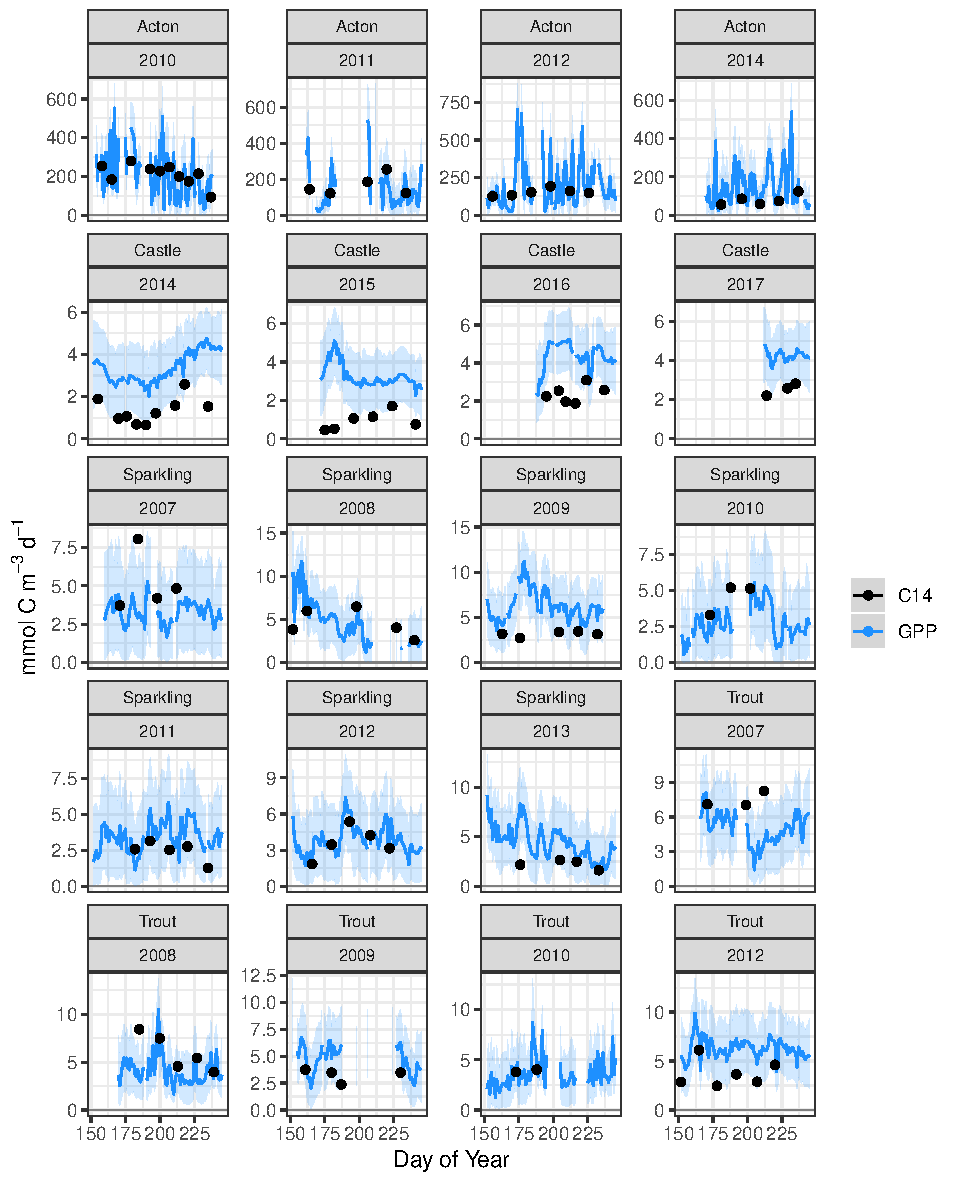
\includegraphics{metabolism.pdf}
\noindent\caption{Time series of pelagic epilimnetic primary production determined from high frequency in situ dissolved oxygen data and discrete measurements of epilimnetic primary production determined from \textsuperscript{14}C incubations in 4 lakes that range in trophic status from ologitrophic to hypereutrophic. Light blue shaded areas represent the 95\% credible interval of the free-water O\textsubscript{2} estimate.}
\label{fig:timeseries}
\end{figure}%---------------------End Figure 1---------------------------------------------%
\newpage

%----------------------------------------------Figure 2----------------------------------------------------%
\begin{figure}
\centering
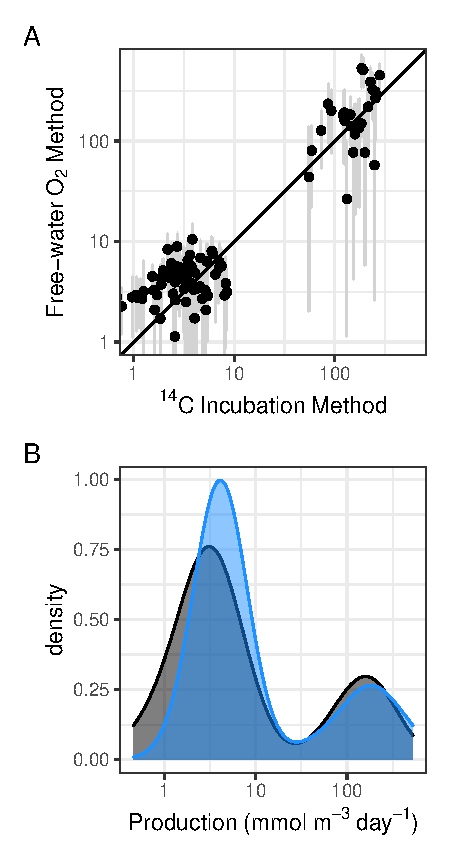
\includegraphics{point_estimates.pdf}
\caption{Point estimate (A) and distribution (B) comparisons of \textsuperscript{14}C and free-water O\textsubscript{2} production (mmol C m\textsuperscript{-3} d\textsuperscript{-1}) estimates from concurrent observations in four lakes of varying trophic status. Error bars (A) are 95\% credible intervals from bayesian metabolism model. (B) Blue is the free-water O\textsubscript{2} estimate, black is the \textsuperscript{14C} estimate. O\textsubscript{2} production values in B are posterior median daily values from Bayesian metabolism model}
\label{fig:pointestimates}
\end{figure}

%----------------------------------------------Figure 3----------------------------------------------------%
\newpage
\begin{figure}
\centering
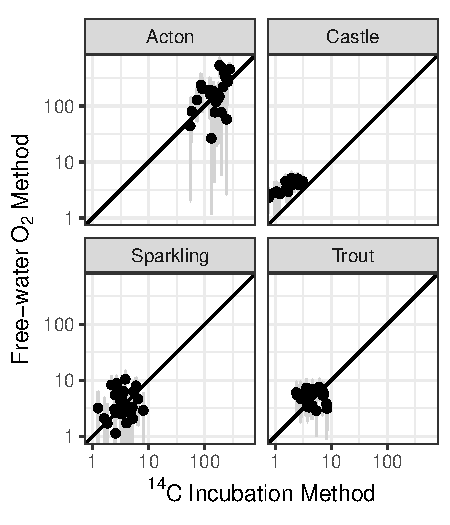
\includegraphics{lake_values.pdf}
\caption{Point estimate comparisons of \textsuperscript{14}C and free-water O\textsubscript{2} production estimates from concurrent observations in four lakes of varying trophic status.}
\label{fig:lakevalues}
\end{figure}
\clearpage

%----------------------------------------------Figure 4----------------------------------------------------%
\newpage
\begin{figure}
\centering
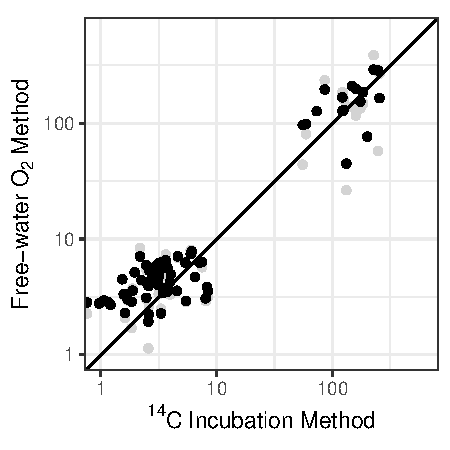
\includegraphics{median_point.pdf}
\caption{Comparison of daiy estimates of \textsuperscript{14}C production and weekly median free-water O\textsubscript{2} production in four lakes of varying trophic status. Light grey points are non-averaged original estimates for each day.}
\label{fig:medianvalues}
\end{figure}
\clearpage

\appendix
\section*{Appendix}
\renewcommand{\figurename}{Appendix}
\setcounter{figure}{0}
\begin{figure}[h]
\centering
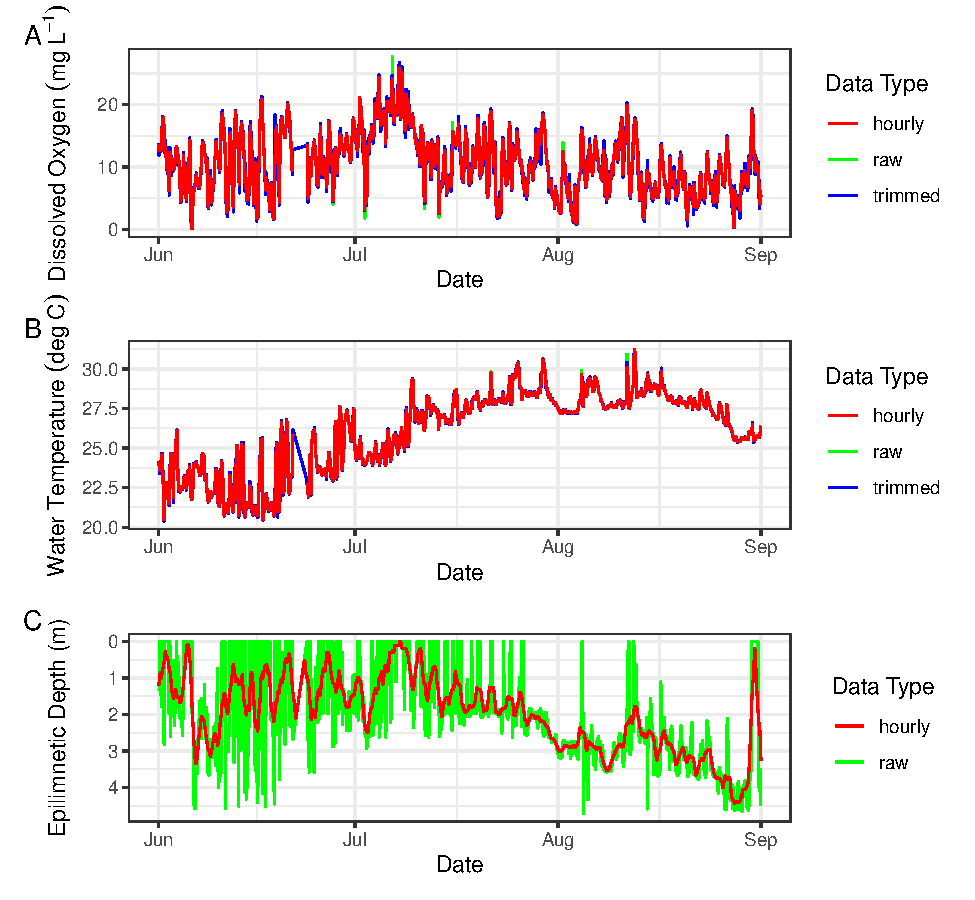
\includegraphics{appendix1.pdf}
\caption{Time series of data from Acton Lake (2010) showing the raw (green), outlier free (blue), and hourly estimates (red) for dissolved oxygen (A), water temperature at a the dissolved oxygen sensor depth (B) and epilimnetic depth or mixed layer depth (C). Hourly values for epilimnetic depth is based on a hourly rolling mean over a 24 hour time period while hourly data in other plots is the simple average value for each discrete hour.}
\label{Appendix:appendix_trimmed}
\vspace{-20pt}
\end{figure}
\clearpage

\end{document}

\endinput
%%